\chapter[大语言模型训练流程]{大语言模型的训练流程}\label{chap:pipeline}

\begin{learningbox}
本章将介绍语言模型的训练方法。具体而言，学完本章后，你将能够：
\begin{itemize}[leftmargin=*, nosep]
    \item 描述基本训练流程的主要阶段，并解释各阶段的目的：{\em 数据获取、预训练、微调、偏好调优与推理}。
    \item 区分{\em 预训练与微调}，并解释为什么偏好调优安排在这两个阶段之后，而非之前。
    \item 解释{\em 编码器与解码器}的区别如何决定模型所采用的训练目标。
    \item 识别评估语言模型的常用{\em 基准测试}，并说明各项基准旨在衡量什么能力。
\end{itemize}
\end{learningbox}

\section{模型训练}

大语言模型（large language model，LLM）的训练流程遵循一套相对标准的方法：首先确定模型架构，并随机初始化参数，随后通过称为{\em 预训练}（pretraining）的过程，训练模型的语言能力。在预训练期间，我们向模型提供大规模文本语料库，让模型以自回归方式进行训练。这一阶段得到的是基础模型，通常还不适合具体的实际应用。因此，我们需要让它适应某个下游任务或用途。这一阶段称为{\em 后训练}（posttraining）：我们向模型提供特定类型的额外数据，借此引导模型表现出针对具体任务的行为，例如遵循指令或完成分类任务。

\subsection{编码器模型与解码器模型}
正如上一章所见，模型主要有两种类型。一方面，编码器模型能够根据输入数据构建丰富的上下文化表示；不过，近期取得的大多数成功都基于解码器模型。编码器更擅长理解任务，例如分类与情感分析；解码器则擅长生成任务。解码器模型的规模不断扩大，可训练参数的数量和可用训练数据的规模都在增长。这使得模型能够以出人意料的能力，泛化到未曾见过的上下文中。

下面，我们将更详细地考察仅解码器模型训练流程中的相关步骤。

\subsection{预训练／微调范式}

当前训练流程取得成功的一个关键特征，是采用了迁移学习（transfer learning）。现代 Transformer 模型的一种标准用法，是选取一个已在大规模通用数据集上训练过的模型，再针对新任务重新训练。模型先在大规模通用语料库上进行{\em 预训练}，然后利用新任务现有的小规模数据集，针对这一具体任务进行{\em 微调}（finetuning）。新任务的微调速度很快，既因为数据集较小，也因为预训练得到的权重已经迁移过来，无须从头开始训练。

迁移学习范式中预训练与微调的区分，是大语言模型训练流程的核心。
模型可以在新情境中复用已经学到的语言知识，从而加快训练过程，无须从头开始。大型商业模型的预训练可能需要数月。新任务通常比较具体，例如特定领域的问答或情感分析。对于新任务，我们会使用专门的数据集来微调模型。在微调过程中，模型的一部分权重会被谨慎更新，使模型在保留预训练所获得的一般语言能力的同时，理解新任务。将模型微调到一个新任务，通常需要数分钟到数小时。

\subsection{开放模型与封闭模型}
\label{sec:pipeline-models}
流行的大语言模型包括 OpenAI 的 ChatGPT 系列 \citep{achiam2023gpt,ouyang2022training}、Meta 的 LLaMa 系列 \citep{touvron2023llama}、Google 的 Gemma \citep{chowdhery2023palm} 与 Gemini \citep{team2023gemini}、Anthropic 的 Claude 系列、Moonshot AI 的 Kimi，以及 DeepSeek \citep{guo2025deepseek} 和 Qwen \citep{bai2025qwen2} 等。

这些模型的开放程度各不相同。例如，模型的训练数据可以公开，网络架构可以披露，训练后的权重也可以发布。不过，商业模型背后的公司为了保持一定的竞争优势，很少会公布模型及其训练过程的全部要素。

为此，科学界开发了完全开源的模型，例如 BLOOM \citep{le2023bloom}、Pythia \citep{biderman2023pythia} 和 OLMo \citep{groeneveld2024olmoacceleratingsciencelanguage}，以增进人们对大语言模型工作原理的共同理解。这些模型训练流程的全部要素都是公开的，也是本章讨论的重点。我们还会介绍某些商业模型的部分特点。

尽管这些模型都基于 Transformer 架构，但各个组件及其整体布局仍存在细微差异，例如，为了利用硬件差异，或采用各自开发者提出的特定优化方法。比如，Google 针对其基于 TPU 的计算基础设施优化了 Gemini \citep{jouppi2023tpu}。第~\ref{chap:scaling}~章将详细讨论架构方面的进一步改进。

\section{训练流程}
\label{sec:pipeline-training}
下面，我们将更详细地介绍标准训练流程的各个步骤。
大语言模型通过包含不同训练阶段的复杂流程构建而成 \citep{radford2019language,minaee2024large}。我们将逐一介绍图~\ref{fig:llm-training-pipeline}~所示的各个阶段。这些阶段的不同组合通常称为训练{\em 配方}（training recipe），它们规定了模型训练各阶段的先后顺序。每个阶段都可能采用新的数据集和新的损失函数。各阶段的设计目的，是赋予模型某种特定能力。在讨论各阶段时，这一点会逐渐清楚。

\begin{figure}
    \centering
    \includestandalone[width=\textwidth]{part1/visuals/tikz/llm_pipeline_overview}
    \caption{大语言模型训练流程概览 \citep{radford2019language,minaee2024large}。}
    \label{fig:llm-training-pipeline}
\end{figure}

\subsection{获取数据}
训练流程的第一步是获取数据。通常，我们会使用海量的通用文本语料库 \citep{brown2020language}。语料库由原始文本构成，无须人工标注。这些数据通常汇集自经过整理和未经整理的在线来源，随后通过启发式清洗方法进一步处理，以减轻有害内容、隐私内容或受版权保护内容的影响。
用于预训练的语料库规模庞大。现代大语言模型使用网络规模的数据进行训练，词元数量往往达到数万亿。以下是一些数据集的例子：

\begin{itemize}
    \item Common Crawl：一个非营利项目提供的海量网页快照，包含数十亿个页面；其他来源还包括 \url{https://archive.org}。尽管其规模无可比拟，数据质量仍存在争议 \citep{baack2024critical}。许多衍生数据集，例如 C4（Colossal Clean Crawled Corpus），提供了经过过滤的英文网络文本子集 \citep{raffel2020exploringc4}，以提高数据质量。
    \item Dolma 3：一种混合数据集，旨在最大化模型在一系列多样化任务上的表现。OLMo 开源／开放数据项目使用了该数据集 \citep{olmo2025olmo3, soldaini2024dolma}。
    \item SmolLM3：采用大规模三阶段训练策略，使用 11.2 万亿个词元，并动态混合网络、数学与代码数据，以优化推理与知识获取 \citep{bakouch2025smollm3}。
\end{itemize}
近期研究强调，对于提升跨领域知识与下游泛化能力而言，数据的多样性与规模同样关键 \citep{gao2020pile800gbdatasetdiverse}。名为{\em The Pile} 的语料库就是专门构建的异质语料库。例如，在 The Pile 上训练的模型，在 GitHub 代码仓库、医学论文与哲学文本等差异很大的领域中，编码效率（每字节比特数，bits per byte，BPB）都有显著改善\footnote{每字节比特数是信息论中一种不依赖词元化器的指标，衡量每个符号平均需要多少比特，反映编码效率，另见第~\ref{sec:metrics}~节。}（见图~\ref{fig:pile}）。因此，它也经常被用作基准测试；模型在 Pile BPB 上取得良好表现，被视为其具备世界知识与复杂推理能力的一项指标。

整理预训练数据，需要制定复杂的数据清洗流程，将来自多个来源的原始数据转化为一组经过清洗的纯文本文档。这一过程通常侧重于质量保证与安全。整理工作首先对来源排定优先级，在混合数据中给予 Wikipedia、图书及其他已知经过整理的优质来源更高权重。随后，为确保语料库的完整性，研究者会采用降噪启发式方法，去除模板文字、导航菜单以及可能不合适的内容。此外，还会在 URL 和文档两个层面去重；这对于防止模型记忆冗余信息、对重复数据过拟合至关重要。

除了准确性，训练流程还必须选择符合安全与伦理约束的数据。这通常也通过基于启发式规则的过滤来实现。此外，还会使用毒性检测系统来去除仇恨言论，不过这些方法的效果往往好坏参半。这一阶段的一大挑战是缓解偏差：自动过滤器可能无意中标记并压制使用特定方言撰写的正当数据，例如非裔美国人英语，从而使训练集意外排除多样化的声音。

\begin{figure}[tb]
    \centering
    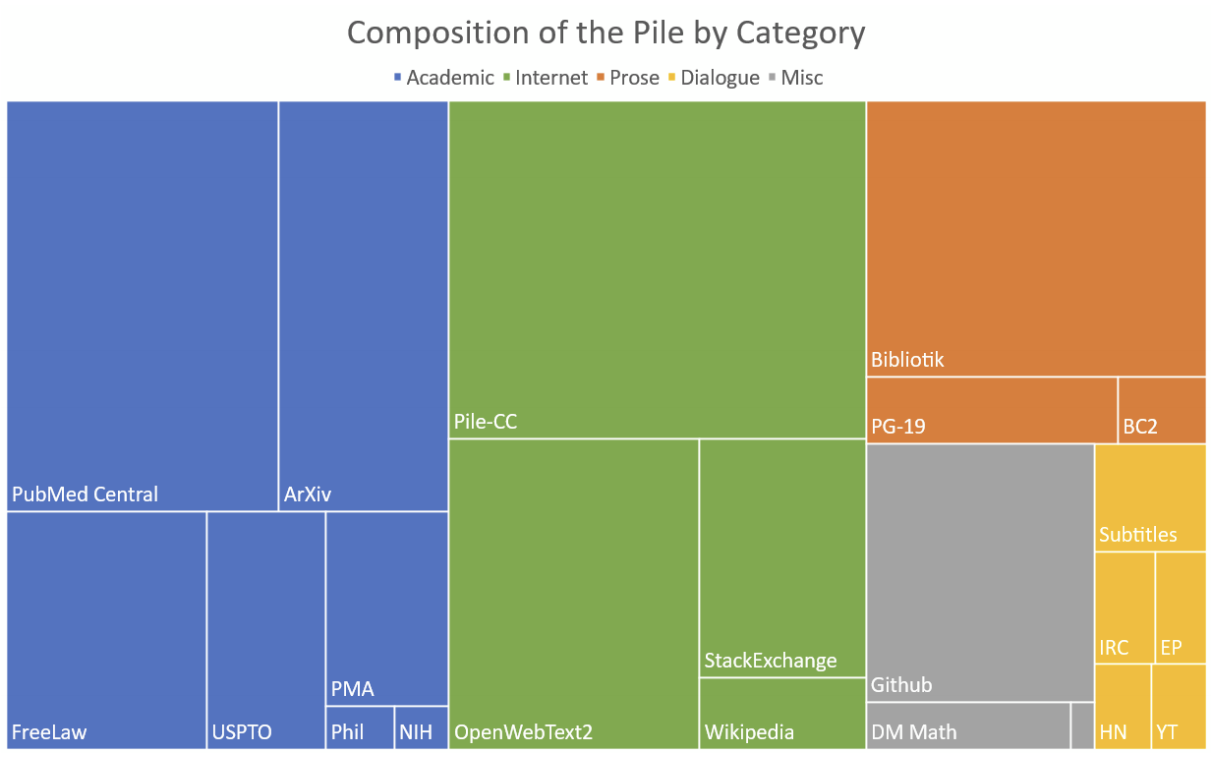
\includegraphics[width=0.9\linewidth]{part1/visuals/the_pile.png}
    \caption{The Pile 数据集中的数据来源概览 \citep{gao2020pile800gbdatasetdiverse}。}
    \label{fig:pile}
\end{figure}

\subsection{预训练}
训练流程的第二步，是在整理好的语料库上预训练模型，由此得到通用自然语言模型。这一阶段对无标注文本采用基于 Transformer 的自监督方法 \citep{vaswani2017attention}。

为了获得语言、概念间语义关系以及世界知识的内部表示，模型通过类似完形填空的掩码词元任务进行训练。
在这类任务中，目标是以大规模序列语料库中的前文为条件，预测被掩码的词元；这些序列可以表示文本或图像块。这一过程采用自监督方式，无须人工标注数据；已知它能够产生丰富的语言表示，以及多种形式的概念间关系与世界知识表示。

形式上，语言建模的目标，是根据包含 $k$ 个已有词元的窗口，最大化句子 $\mathcal{U} = \{u_{0}, \dots, u_{n} \}$ 中词元的概率（式~\ref{eq:lm}）。$L(\mathcal{U})$ 为{\em 语言建模损失}。

\begin{equation}
\label{eq:lm}
    L(\mathcal{U}) = \sum_i \log P(u_i | u_{i-k}, \dots, u_{i-1}; \Theta)
\end{equation}

语言模型通过可训练参数 $\Theta$ 来估计这些概率，并通过梯度更新来优化参数。由于模型的规模从数百万参数到超过一万亿参数不等，需要大规模数据集才能确保收敛。在这一训练阶段，模型采用教师强制（teacher forcing）：模型作出预测后，下一步输入的是真实词元，而不是模型自身的输出。相比之下，在推理阶段进行自回归生成时，模型必须依赖自身的预测，作为生成后续词元的输入。词元由相应的{\em 词元化器}生成，第~\ref{sec:tokenization}~节已作介绍。

预训练的一个关键挑战，是确保模型高效学习，并在数万亿次梯度更新的整个过程中保持稳定。随着时间推移，人们发展出不同策略，力求控制训练过程。其中一种策略是课程学习（curriculum learning）。人类学习时，先学习简单概念，例如加法，再学习较难的概念，例如乘法与对数。在语言建模中，这一思路体现为数据混合或数据课程。研究者不会同时使用所有类型的数据进行训练，而是先选定特定的数据来源组合，参见图~\ref{fig:smollm3-mixture}~中的例子。构建混合数据时，需要按难度有策略地安排数据顺序。在训练课程中，我们先使用容易学习的通用网络抓取数据，再在后续阶段转向更难、质量更高的推理数据，例如数学与代码数据。其基本思路是，这有助于模型在更复杂的逻辑上更快收敛 \citep{bengio2009curriculum}。

\begin{figure}[tb]
    \centering
    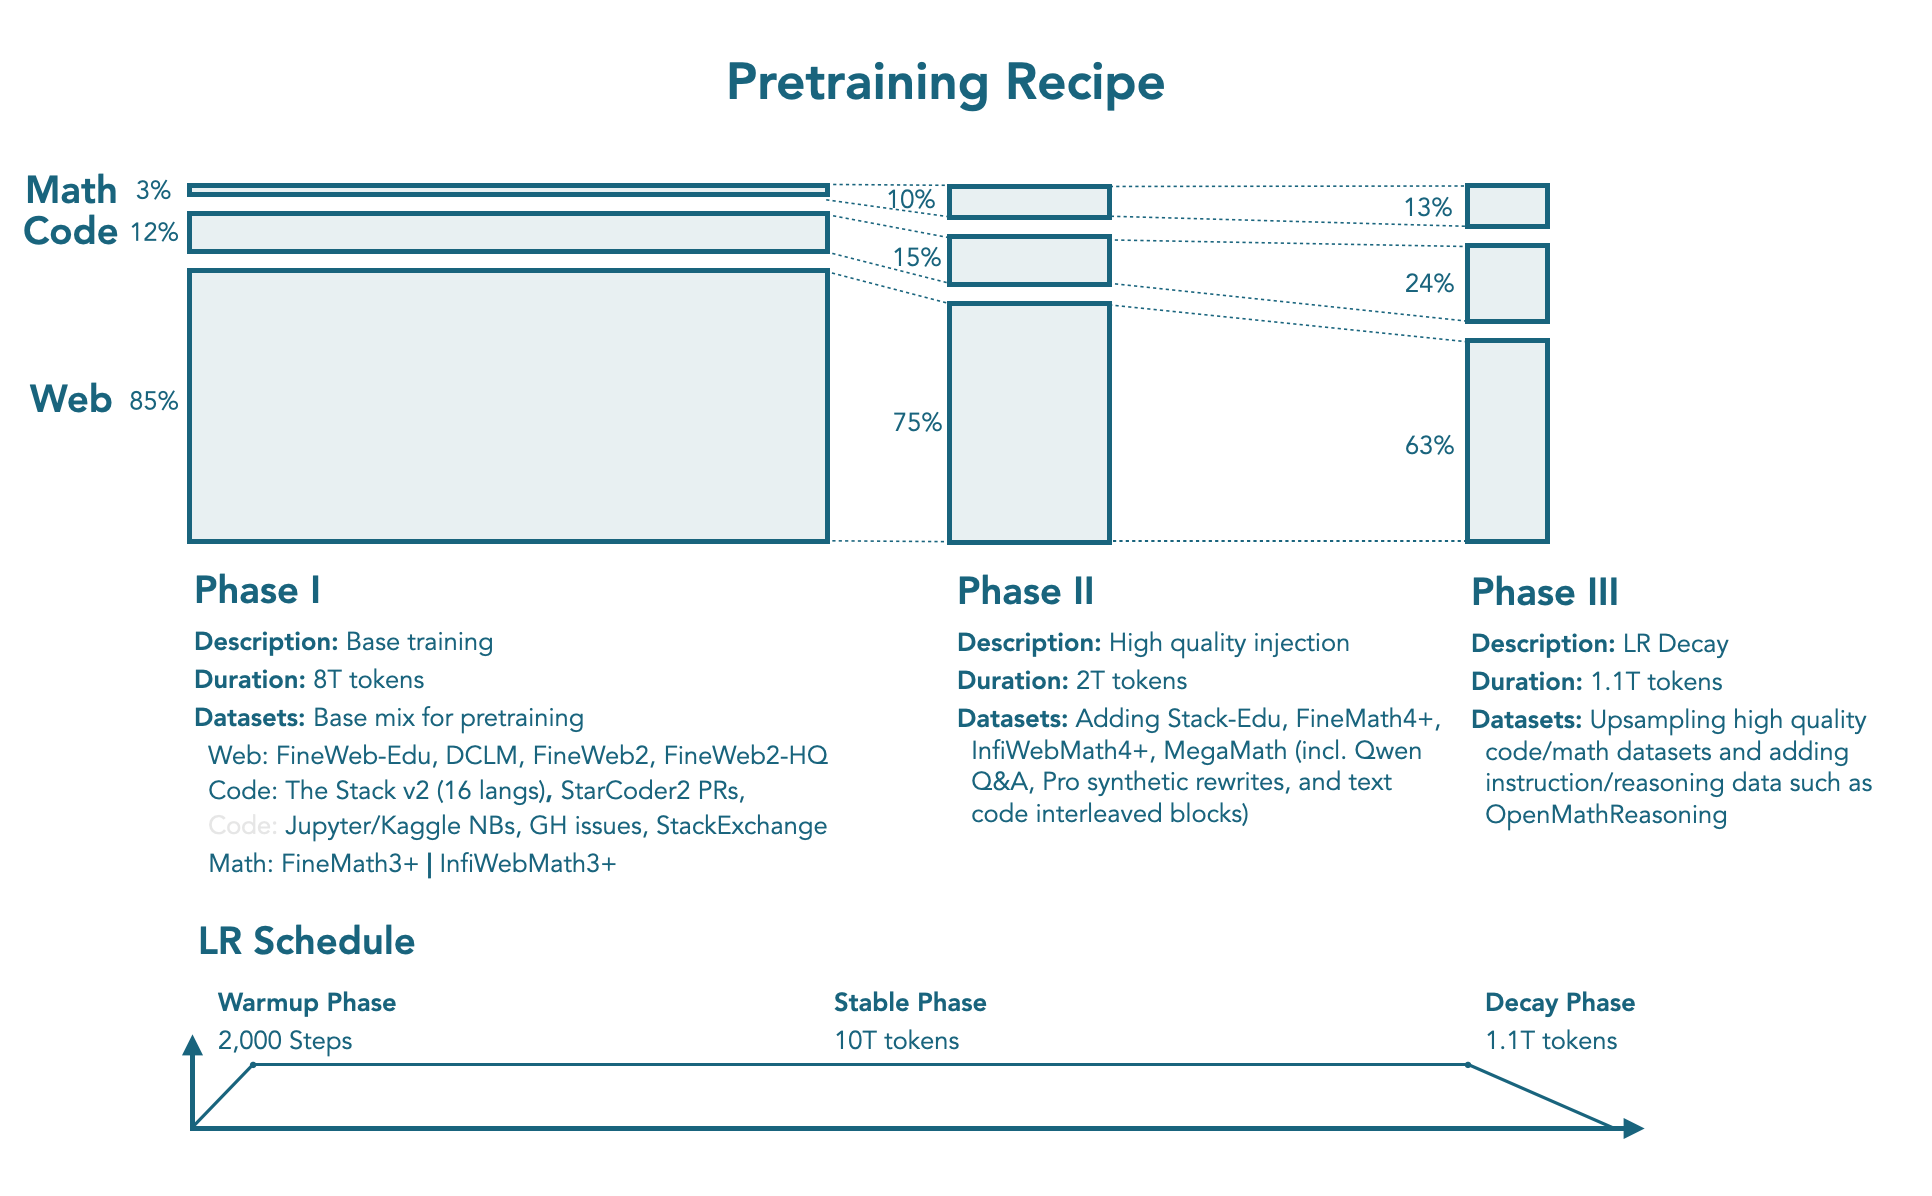
\includegraphics[width=\linewidth]{part1/visuals/smollm3_mixture.png}
    \caption{用于训练 SmolLM3 的混合数据示例 \citep{bakouch2025smollm3}。}
    \label{fig:smollm3-mixture}
\end{figure}

人们还会采用其他机制来稳定训练，因为这一规模的训练极不稳定，容易出现损失突增（loss spike）\citep{takase2025spikemorestabilizingpretraining}。权重衰减、层归一化以及精细的学习率调度器等标准机器学习技术，可用于维持训练稳定性。使用专门的优化器并监测梯度范数，有助于防止参数在高强度预训练过程中发散。图~\ref{fig:glm-spike}~展示了一个例子，说明调整嵌入层如何使训练更加稳定。左图给出 3.36 亿参数与 7.52 亿参数 BERT 模型的训练损失。原始架构在 3.36 亿参数模型上表现良好，而图 (b) 中的修改能够实现稳定训练，并获得更低的训练损失 \citep{shoeybi2020megatronlmtrainingmultibillionparameter}。

\begin{figure}[tb]
    \centering
    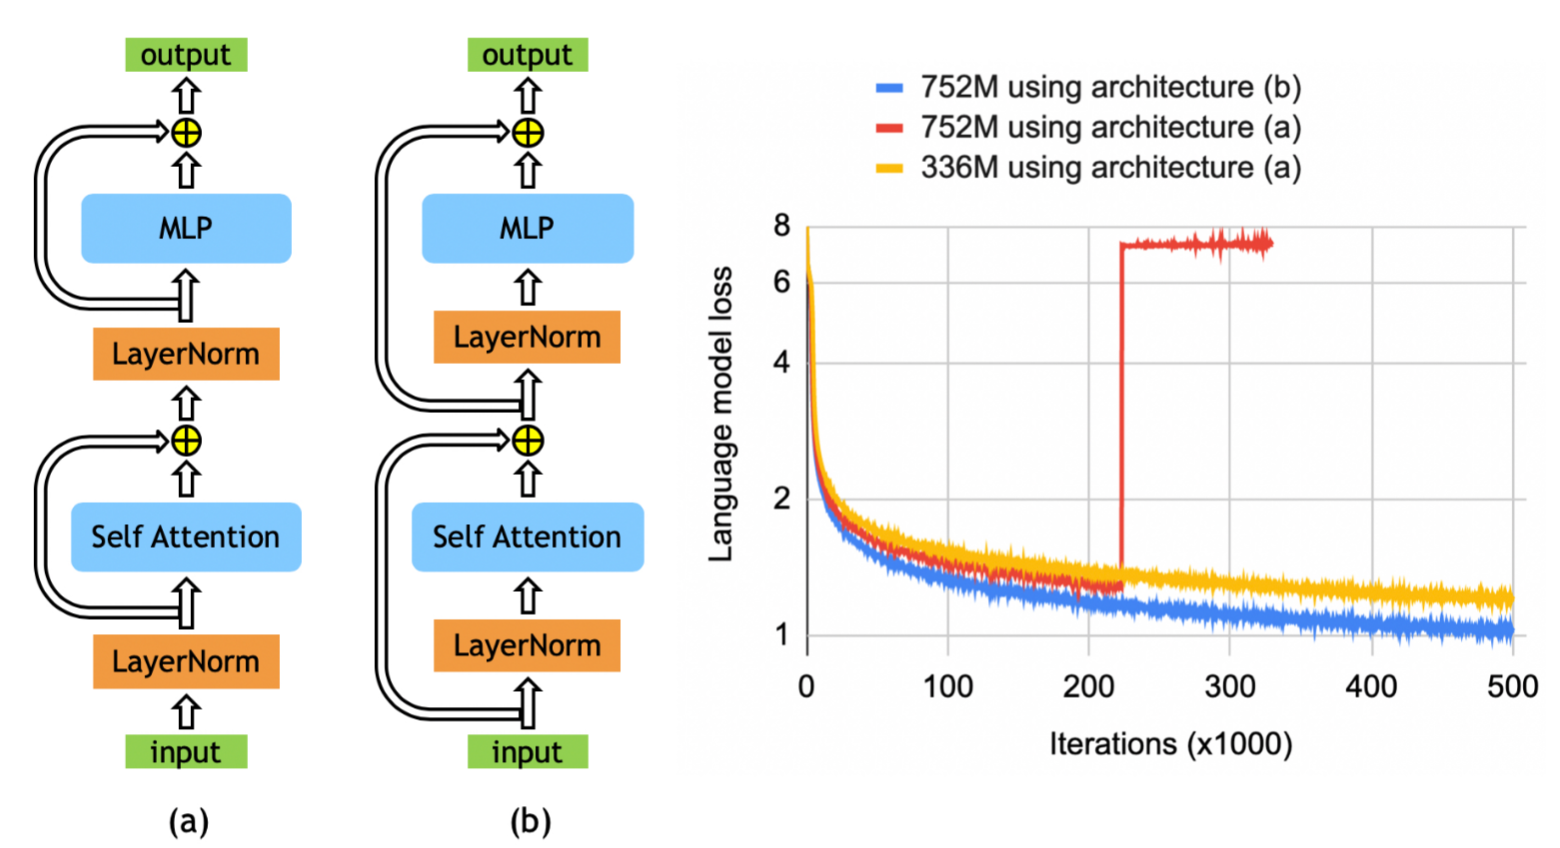
\includegraphics[width=0.9\linewidth]{part1/visuals/glm_spike.png}
    \caption{采用原始架构 (a) 与调整后架构 (b) 的 BERT 模型训练损失 \citep{shoeybi2020megatronlmtrainingmultibillionparameter}。
    }
    \label{fig:glm-spike}
\end{figure}

\subsection{微调}
预训练之后是后训练，其中第一个重要的训练步骤是微调。
人们很少将大语言模型仅仅用于通用的自动补全，也就是预测下一个词，而是用它来回答问题、提供建议和回忆信息。微调，是指选取一个已经学会一般语言模式的预训练模型，再在规模较小、更为专门的数据集上进一步训练。在微调中，我们采用监督学习方法，利用有标注数据集，将通用模型用于某项具体而狭窄的任务。
一种流行的高效方法是低秩优化，它只微调一小部分参数 \citep{hu2021lora,wei2022emergent,minaee2024large}。

\paragraph{监督微调（SFT）}
微调可以用于许多专门任务。最通用的模型会采用{\em 监督微调}（supervised finetuning，SFT），以便遵循指令并执行推理步骤 \citep{olmo2025olmo3}。监督微调对较小的模型尤为重要：它提供了一种高效机制，能够显著改善通用聊天、推理与函数调用能力。

监督微调也用于更专门的任务，例如降低毒性。WildChat \citep{zhao2024wildchat} 提供了超过一百万次真实用户与 ChatGPT 的交互，记录了人类如何用复杂程度与毒性各异的提示来使用大语言模型。

在学习推理能力方面，OpenThoughts \citep{guha2025openthoughts} 包含从先进模型中蒸馏得到的逐步推理链，以增强模型在数学、科学与编程方面解决问题的能力。除了从人类获取的数据，还会补充合成数据（synthetic data）：利用更大的教师模型，例如 GPT-5，生成指令与回答，以填补特定数据缺口并扩大训练量 \citep{zhang2026instruction}。

微调并不仅限于一般的指令遵循或推理。其他任务还包括不同语言之间的翻译，或医疗与客户服务领域的问答。尤其是在任务范围狭窄、模型规模较小的工业应用中，微调是一种卓有成效的做法。

第~\ref{sec:tools}~章将讨论大语言模型对工具的使用，这是智能体大语言模型的一个核心方面。工具使用能力的训练，也发生在训练流程中的监督微调阶段 \citep{wei2022emergent,minaee2024large}。

此外，微调对于塑造模型的人格特征、深化其专业能力也很重要。例如，组织可以训练模型采用某种特定的表达语气，让客服机器人保持一致的品牌形象：可以是善解人意、正式庄重，也可以是机智诙谐、轻松随意。最后，注入深入的领域知识，可以使模型掌握细分领域中复杂的术语与逻辑，例如行业专利信息，或专有遗留代码的调试。

最终，微调将通用预测器转化为专门领域的专家，往往使规模更小、效率更高的模型，能够在特定任务上胜过更大的基础模型。

\subsection{偏好调优}
早期模型暴露出一个问题：训练往往会放大训练数据中极端且不为社会所接受的文本，使其失去控制，并挤压温和观点的空间。此后，为使大语言模型的行为能够被社会接受，训练流程必须包含一个阶段，专门将模型调优到社会能够接受的行为方式。这一阶段称为偏好调优（preference tuning）。

在这一阶段，我们使微调后的模型与用户期望保持一致，即进行偏好对齐（preference alignment）。这一步旨在改进模型，使其给出社会能够接受的回答、防止仇恨言论、减少幻觉，并更好地遵循指令。

偏好调优的标准方法包括基于人类反馈的强化学习（reinforcement learning from human feedback，RLHF）\citep{ouyang2022training}，它训练奖励模型来近似人类价值观；以及直接偏好优化（direct preference optimization，DPO）\citep{rafailov2024direct}，它直接利用偏好数据优化策略。图~\ref{fig:rlhf-loop}~给出了 RLHF 的总体概览。为缓解人工标注的瓶颈，现代训练流程越来越多地采用基于 AI 反馈的强化学习（reinforcement learning from AI feedback，RLAIF）\citep{bai2022constitutional}，由更强大的模型生成偏好信号。

\begin{figure}[tb]
    \centering
    \begin{tikzpicture}[
    x=1cm,y=1cm,>=Latex,font=\small,
    card/.style={draw=black!35,minimum width=.78cm,minimum height=.8cm,inner sep=3pt,font=\large},
    model/.style={draw=black!45,rounded corners=5pt,minimum height=1cm,align=center,inner sep=6pt},
    flow/.style={->,thick}
]
    \draw[densely dashed,black!55] (5.4,0) -- (5.4,5.8);
    \node[font=\bfseries] at (2.5,5.45) {偏好数据};
    \node[card,fill=cyan!45] (px) at (.6,4.3) {$x$};
    \node[card,fill=yellow!75!orange] (pa) at (1.9,4.3) {$a^1$};
    \node[card,fill=yellow!75!orange] (pb) at (3.2,4.3) {$a^2$};
    \node[card,fill=violet!35] (py) at (4.5,4.3) {$y$};
    \node[text=cyan!55!black] at (.6,3.6) {提示};
    \node[text=orange!80!black] at (2.55,3.6) {回答};
    \node[text=violet!70!black] at (4.5,3.6) {偏好};
    \node[model,fill=green!45,minimum width=2.8cm,font=\bfseries] (rewardleft) at (2.55,1.35) {奖励模型};
    \draw[flow] (2.55,3.15) -- node[right] {训练} (rewardleft.north);
    \node[font=\bfseries] at (2.55,.2) {奖励建模};

    \node[card,fill=cyan!45] (x) at (8.2,5.05) {$x$};
    \node[anchor=west] at (8.85,5.05) {提示集合};
    \node[model,fill=yellow!55,minimum width=3.25cm] (policy) at (8.2,3.65)
        {\textbf{策略模型}\\[-1pt]\footnotesize 待对齐的大语言模型};
    \draw[flow] (x.south) -- (policy.north);
    \node[card,fill=yellow!75!orange] (a) at (7.55,1.35) {$a^1$};
    \node[card,fill=yellow!75!orange] (b) at (8.85,1.35) {$a^2$};
    \draw[flow] (policy.south) -- node[right] {生成回答} (8.2,1.95);
    \node[model,fill=green!45,minimum width=2.4cm,font=\bfseries] (reward) at (13.05,1.35) {奖励模型};
    \draw[flow] (9.55,1.35) -- (reward.west);
    \node[card,fill=violet!35] (y) at (13.05,3.65) {$y$};
    \draw[flow] (reward.north) -- node[right] {输出偏好} (y.south);
    \draw[flow] (y.west) -- node[above] {更新参数} (policy.east);
    \node[font=\bfseries] at (10.5,.2) {在线迭代 RLHF};
\end{tikzpicture}

    \caption{RLHF 总体概览：训练奖励模型（左），并依据该奖励模型优化语言模型（策略），参见 \citet{dong2024rlhf}。}
    \label{fig:rlhf-loop}
\end{figure}

实现与人类价值观的对齐并非易事。通常，我们区分安全对齐、价值对齐与偏好对齐。对于偏好对齐，一个复杂之处在于，偏好带有主观性，例如写作风格，不同人的偏好各不相同。

\paragraph{价值对齐}
从更高层面看，价值对齐（value alignment）侧重于确保模型的基本原则与世界观符合广泛的人类伦理。与个人偏好不同，这涉及将模型锚定于公平、有益、诚实等高层次概念。在实践中，这意味着用一套书面原则，即一部{\em 宪法}（constitution），来约束模型，确保其遵守开发者制定的规则。

然而，这种价值对齐通常会带来权衡：为安全性与有用性而优化模型，也会降低其在事实回忆或创造力等其他能力上的表现 \citep{lin2024mitigating}。这种权衡也称为{\em 对齐代价}（alignment tax）。

\paragraph{安全对齐}
安全对齐（safety alignment）是为模型行为设定硬性边界，以防止产生灾难性或有害输出的过程。偏好对齐可能侧重于语气，价值对齐侧重于观点，而安全对齐侧重于对抗鲁棒性以及拒绝恶意提示。保障安全的方法包括红队测试（red teaming）：对模型开展严格的越狱尝试，以发现漏洞；以及设置护栏（guard railing）：针对高风险回答设定明确的拒绝边界，并进行过滤。

\paragraph{客观正确性对齐}
最后，对于数学或编程等存在客观真值的领域，人们采用可验证奖励强化学习（reinforcement learning with verifiable rewards，RLVR）\citep{lambert2024tulu}。与标准 RLHF 不同，RLVR 利用真实答案信号，以客观正确性为优化目标，稳健地提升推理能力。例如，代码能够编译通过，或数学解答正确。在后者中，经常使用组相对策略优化（group relative policy optimization，GRPO）算法 \citep{guo2025deepseek}。它是近端策略优化（proximal policy optimization，PPO）的一种变体，能够增强数学推理能力，同时优化 PPO 的内存使用。具体做法是从策略模型中采样多个答案，利用验证器评估其相对质量，并据此计算奖励。模型不再依赖人工标签来学习什么是好答案，而是直接从确定性验证器获得奖励（+1 或 -1）\citep{guo2025deepseek, shao2024deepseekmath}，见图~\ref{fig:grpo}。

\begin{figure}[tb]
    \centering
    \begin{tikzpicture}[
    x=.97cm,y=.88cm,>=Latex,font=\small,
    trained/.style={draw=blue!40!black,thick,rounded corners=4pt,fill=yellow!18,minimum width=1.55cm,minimum height=.8cm,align=center},
    frozen/.style={trained,fill=blue!10},
    quantity/.style={draw=black!75,rounded corners=2pt,fill=white,minimum width=.85cm,minimum height=.6cm,font=\large},
    flow/.style={->,semithick}
]
    \node[font=\bfseries\large,anchor=west] at (0,7.1) {PPO};
    \node[quantity] (pq) at (.45,5.5) {$q$};
    \node[trained] (pp) at (2.2,5.5) {策略模型};
    \node[quantity] (po) at (3.95,5.5) {$o$};
    \node[frozen] (pref) at (5.9,7.05) {参考模型};
    \node[frozen] (prm) at (5.9,5.95) {奖励模型};
    \node[trained] (pvm) at (5.9,4.85) {价值模型};
    \node[font=\large,inner sep=0pt] (plus) at (7.55,6.55) {$\oplus$};
    \node[quantity] (pr) at (8.65,6.55) {$r$};
    \node[quantity] (pv) at (8.65,4.85) {$v$};
    \node[quantity,font=\normalsize] (gae) at (10.3,5.5) {GAE};
    \node[quantity] (pA) at (11.8,5.5) {$A$};
    \draw[flow] (pq) -- (pp);
    \draw[flow] (pp) -- (po);
    \draw[flow] (po.east) to[out=0,in=180] (pref.west);
    \draw[flow] (po.east) to[out=0,in=180] (prm.west);
    \draw[flow] (po.east) to[out=0,in=180] (pvm.west);
    \draw[flow] (pref.east) to[out=0,in=150] node[above,near start,font=\small] {$KL$} (plus);
    \draw[flow] (prm.east) to[out=0,in=210] (plus);
    \draw[flow] (plus) -- (pr);
    \draw[flow] (pvm) -- (pv);
    \draw[flow] (pr.east) to[out=0,in=150] (gae.west);
    \draw[flow] (pv.east) to[out=0,in=210] (gae.west);
    \draw[flow] (gae) -- (pA);
    \draw[flow] (pA.north) .. controls (11.8,8.3) and (3.2,8.3) .. (pp.north);
    \draw[flow] (gae.south) .. controls (10.3,4.05) and (7,4.05) .. (pvm.south);

    \draw[dashed,thick,black!45] (0,4.1) -- (12.65,4.1);
    \node[font=\bfseries\large,anchor=west] at (0,3.5) {GRPO};
    \node[quantity] (gq) at (.45,1.5) {$q$};
    \node[trained] (gp) at (2.2,1.5) {策略模型};
    \fill[black!5,rounded corners=5pt] (3.35,-.02) rectangle (4.55,3.05);
    \node[quantity] (go1) at (3.95,2.6) {$o_1$};
    \node[quantity] (go2) at (3.95,1.65) {$o_2$};
    \node[font=\large] at (3.95,.9) {$\cdots$};
    \node[quantity] (goG) at (3.95,.35) {$o_G$};
    \node[frozen] (gref) at (5.9,2.65) {参考模型};
    \node[frozen] (grm) at (5.9,1.5) {奖励模型};
    \fill[black!5,rounded corners=5pt] (7.7,-.02) rectangle (8.9,3.05);
    \node[quantity] (gr1) at (8.3,2.6) {$r_1$};
    \node[quantity] (gr2) at (8.3,1.65) {$r_2$};
    \node[font=\large] at (8.3,.9) {$\cdots$};
    \node[quantity] (grG) at (8.3,.35) {$r_G$};
    \node[draw=blue!40!black,rounded corners=4pt,align=center,minimum width=1.25cm,minimum height=.85cm] (group) at (10.15,1.5) {组内计算};
    \fill[black!5,rounded corners=5pt] (11.2,-.02) rectangle (12.4,3.05);
    \node[quantity] (gA1) at (11.8,2.6) {$A_1$};
    \node[quantity] (gA2) at (11.8,1.65) {$A_2$};
    \node[font=\large] at (11.8,.9) {$\cdots$};
    \node[quantity] (gAG) at (11.8,.35) {$A_G$};
    \draw[flow] (gq) -- (gp);
    \draw[flow] (gp.east) -- (3.35,1.5);
    \draw[flow] (4.55,1.5) to[out=0,in=180] (gref.west);
    \draw[flow] (4.55,1.5) -- (grm.west);
    \draw[flow] (grm.east) -- (7.7,1.5);
    \draw[flow] (8.9,1.5) -- (group.west);
    \draw[flow] (group.east) -- (11.2,1.5);
    \draw[flow] (gref.north) .. controls (5.9,3.5) and (3.0,3.55) .. node[above,pos=.38] {$KL$} (gp.north);
    \draw[flow] (11.8,3.05) .. controls (11.8,4.05) and (3.0,4.05) .. (gp.north);

    \fill[black!5,rounded corners=6pt] (13.05,2.7) rectangle (15.0,6.4);
    \node[trained,minimum width=1.6cm,align=center] at (14.02,5.5) {训练中的\\模型};
    \node[frozen,minimum width=1.6cm,align=center] at (14.02,3.7) {冻结的\\模型};
\end{tikzpicture}

    \caption{RLHF 方法（具体为 PPO）与 RLVR 方法（具体为 GRPO）的比较 \citep{shao2024deepseekmath}。}
    \label{fig:grpo}
\end{figure}

\subsection{推理}
训练流程的最后一步是推理，也就是训练完成的模型终于投入使用的阶段。
在这里，用户终于可以与模型交互，我们也终于能够使用训练工作的成果。

在推理阶段，我们使用自然语言提示，即指令与问题，来获取模型的回答。让大语言模型回答问题时，提示是首选的使用方式。推理结果可能对提示的表述方式十分敏感。在提示中使用某些词语，或改变词语顺序，都可能影响模型的回答。这种敏感性催生了提示工程（prompt engineering）与上下文工程（context engineering），它们已经成为大语言模型用户的重要技能 \citep{sahoo2024systematic}。

有趣的是，正如上一章所述，当解码器模型的规模超过数千亿参数时，一种新的学习方法便会涌现：{\em 上下文学习}（in-context learning，ICL）\citep{brown2020language,wei2022emergent}。上下文学习是指在提示中同时给出少量示例与一条指令。这些示例为模型指明某个方向，模型利用它们学习如何作答。ICL 是一种在提示内部进行的少样本学习。ICL 还是一种不改变模型任何参数的学习方式，即通过示例学习，却不进行参数训练 \citep{dong2022survey}。

在本书后续内容中，我们会看到许多上下文学习的应用实例，例如智能体控制框架中的用法。推理阶段的上下文学习，是智能体大语言模型发展的主要驱动力之一。

\subsection{小结}
我们已经介绍了典型大语言模型训练流程的各个阶段。
请注意，这里所描述的流程只是典型方法的一个例子，不同模型的训练方式有所不同。当前的现代训练流程十分复杂，训练成本也很高。训练流程的创新是当前研究的主题，例如可参见 \citet{guo2025deepseek,team2025kimi}。

快速获得预测结果至关重要，人们也已开发出多种技术来加快这一过程。例如，在推理投入与回答质量之间取得平衡很重要。{\em 测试阶段扩展}（test time scaling）研究的就是这一权衡。推理阶段投入越多，消耗的计算时间也越多，但可能得到更好的答案。第~\ref{chap:scaling}~章将讨论这些技术及其他优化方法。

\section{基准测试与性能}
\label{sec:pipeline-benchmarks}
通过训练流程训练好模型之后，我们希望了解模型的表现究竟如何。
大语言模型采用多种建模技术，针对不同任务、在不同数据集上构建而成。因此，它们往往获得了引人注目的能力。例如，大语言模型在自然语言理解任务（GLUE、SQUAD、Xsum）\citep{wang2018glue,wang2019superglue,rajpurkar2016squad,narayan2018don}、翻译 \citep{kocmi2022findings,papineni2002bleu,sennrich2015improving}、问答任务 \citep{roberts2020much} 以及诗歌创作 \citep{zhang2024llm} 等领域都有良好表现，这里仅列举了少数几个领域。广泛的适用性体现了大语言模型的多才多能；不过，领域的快速发展与持续的研究工作，也提出了许多尚待回答的问题，涉及大语言模型在众多领域与情境中的能力。

下面，我们将讨论一些常用于测试模型性能的基准。

\subsection{常见任务}
我们来更仔细地考察一些常见的大语言模型任务。这些任务大体可以归入此前介绍的两类语言处理任务：自然语言理解（natural language understanding，NLU）与自然语言生成（natural language generation，NLG）。
具体采用什么性能指标，取决于任务类别、准确的任务表述及其所用数据。我们将分别讨论。

请注意，{\em 性能}（performance）一词具有歧义。在自然语言处理中，它通常指\emph{任务表现}，即准确性，而不是\emph{计算性能}，即速度。虽然准确的评估标准随任务而异，现代评估实践主要关注任务表现。不过，要在当今的基准测试中取得高分，我们调用大语言模型的次数，以及从模型获得回答的速度，也同样重要；后续章节将会介绍这一点。

\subsection{指标}\label{sec:metrics}
为了监测或报告大语言模型的任务表现，我们会根据所处的训练阶段使用不同指标。

\paragraph{预训练指标}
在预训练阶段，我们最关心的是模型能否准确预测下一个词。标准指标是{\em 困惑度}（perplexity），如式~\ref{eq:perplexity}~所示。困惑度衡量模型预测下一个词元时的不确定性，与交叉熵损失函数直接相关。低困惑度表明，模型为正确的后续词元赋予了较高概率。困惑度越低越好。

\begin{equation}
    \text{PPL}(X) = \exp \left( - \frac{1}{N} \sum_{i=1}^N \log P(x_i \mid x_{<i}) \right)
    \label{eq:perplexity}
\end{equation}

\begin{equation}
    \text{BPB} = - \frac{1}{B} \sum_{i=1}^N \log_2 P(x_i \mid x_{<i})
    \label{eq:bits-per-byte}
\end{equation}
困惑度是在词元上计算的；若要调整困惑度，使其遵循单词边界，就需要谨慎归一化 \citep{pimentel-meister-2024-compute}。而且，即使经过调整，它仍依赖具体的词元化器，因为其他词元化器可能产生不同的子词，进而得到不同的概率分布。

另一种指标是\emph{每字节比特数}（BPB），见式~\ref{eq:bits-per-byte}。它将损失归一化到字节层面，从而能够公平比较采用不同词元化方案的模型 \citep{borgeaud2022improving}。它衡量编码单个字节的数据所需的平均比特数。

\paragraph{后训练指标}
在后训练与推理阶段，模型用于解决问题、生成内容或推理时，我们会根据真实答案数据，考察能够确定判分的成功率。任务通常采用多项选择问答的形式，其中只有一个正确答案。对于这类任务，我们通常报告{\em 准确率}（accuracy），即回答正确的问题所占的百分比。准确率越高越好。

在通常的设置中，模型需要在一次尝试中给出答案。不过，由于从语言模型中采样是一个随机过程，我们可以要求模型多尝试几次，看看其中是否包含正确答案。{\em Pass@K} 指标对此作了形式化定义：它表示模型在第 $K$ 次尝试时正确解决的问题所占的百分比，越高越好。$K$ 的常见取值包括 1、5、10 和 100。

\subsection{常用基准测试}
尽管如何衡量大语言模型的性能仍是一个活跃的研究领域，许多数据集已经成为报告模型一般能力时的常用工具。这些数据集的设计用途仅限于{\em 评估}模型质量，并不打算用作额外的训练数据。因此，它们充当半标准化的基准。MLCommons \citep{thiyagalingam2022ai} 等持续推动建立领域标准的工作，表明人们越来越需要客观、可靠的评估设置。

\begin{table}[tb]
    \centering
    \setlength{\tabcolsep}{4pt}
    \begin{tabular}{@{}>{\raggedright\arraybackslash}p{.18\textwidth}>{\raggedright\arraybackslash}p{.30\textwidth}>{\raggedright\arraybackslash}p{.28\textwidth}>{\raggedright\arraybackslash}p{.18\textwidth}@{}}
        \toprule
        \textbf{基准名称} & \textbf{测试能力} & \textbf{任务形式} & \textbf{指标} \\
        \midrule
        \textbf{Humanity's Last Exam (HLE)} & 通用智能、多模态推理 & 简答、多项选择 & Pass@1 \\
        \textbf{Abstract Reasoning Challenge (ARC)} & 通用智能 & 视觉网格模式补全 & Pass@1（私有测试集） \\
        \textbf{GPQA Diamond} & 专家级科学、技术、工程与数学推理 & 多项选择 & Pass@1 \\
        \textbf{AIME 2025} & 高难度数学推理 & 整数答案（0--999） & Pass@1 \\
        \textbf{SWE-Bench} & 智能体编程、现实世界的软件工程 & 生成代码补丁 & Pass@1 \\
        \textbf{Fortress} & AI 安全、国家安全风险评估 & 多种形式（专有） & 平均风险得分（ARS）与过度拒绝得分（ORS） \\
        \textbf{MMLU} & 广泛的通用知识 & 多项选择 & Pass@1 \\
        \textbf{GSM8K} & 小学数学推理 & 多步算术 & Pass@1 \\
        \textbf{TruthfulQA} & 事实正确性、幻觉检测 & 问答 & Pass@1 \\
        \bottomrule
    \end{tabular}
    \caption{常用大语言模型基准及其报告指标概览。}
    \label{tab:llm-benchmarks}
\end{table}

\paragraph{数据污染}
现代基准面临数据污染（data contamination）的风险~\citep{balloccu-etal-2024-leak}。
随着预训练数据规模增大，往往已占互联网总规模的相当大一部分，领域内与领域外数据之间的界线变得越来越模糊；尤其是商业供应商出于商业利益或其他原因，往往不说明训练数据的来源。因此，如果我们希望衡量模型对未见数据的真实泛化能力，就必须确保模型以前没有见过这些数据，也就是要防止{\em 数据污染}。

常见做法是，基准提供一个公开、可自由访问的数据集，方便开发者快速实验，同时保留一个限制商业供应商访问的私有数据集，以防数据污染。此外，为了让基准在未来继续有用，开发者还经常主动更新其中的样本。

表~\ref{tab:llm-benchmarks}~给出了一份非穷尽的通用基准清单，这些基准在本书写作时较为流行。

\section{结语}

在大语言模型开发领域，商业大语言模型开发者，例如 Anthropic、OpenAI、Google、DeepSeek 和 Mistral，通常会发布技术报告，向专业读者介绍模型在流行基准上的表现。这类技术报告往往以预印本形式发表，未经学术同行评审；出于商业原因，完全实现科学可复现所需的许多细节，例如数据配方与模型架构，也会被省略。尽管如此，这些报告仍提供了有用信息，帮助我们理解大语言模型能做什么、不能做什么。

首先，我们发现，现代大语言模型在不同基准上呈现出明显的能力层次差异：它们实际上已经解决了广泛的知识任务，但在掌握复杂推理与自主智能体任务方面仍有困难。在静态知识与专业考试基准，例如 MMLU 和 TruthfulQA 上，截至本书写作时，前沿模型，例如 GPT-5.2、Gemini 3 Pro 与 Claude 4.5 Opus，已经接近饱和，得分持续超过 85--90\%，并超过人类专家基线。

最新一代推理模型，例如 OpenAI 的 o1、DeepSeek-R1 与 Qwen-3.5，近期取得了巨大进步，将数学与科学任务的通过率从很低的百分比提升到了专家水平。尽管取得了这些进展，软件工程基准 SWE-bench 仍然是可靠性的终极压力测试：顶尖编程智能体的得分，虽然已从微不足道的水平（低于 2\%）提高到相当可观的水平（在经过验证的子集上达到 40--50\%），但从回答编程问题到自主修复现实代码仓库中的问题，两者之间的差距仍是现代 AI 面临的一大障碍。

\paragraph{开放问题}
关于大语言模型能力的来源，仍有许多开放问题。训练流程已经变得复杂：训练阶段涉及{\em 哪些数据重要？哪些训练步骤最重要？}，推理阶段则涉及{\em 如何提取高质量的推理轨迹？}。在这种情况下，很难得出结论。例如，预训练与后训练哪一个更重要，知识是否主要来自预训练，而后训练只负责找到良好的任务接口，仍是开放问题 \citep{zhou2023lima}。

本书后续各部将讨论后训练、推理阶段的推理方法，以及智能体训练方法。不过在此之前，我们将在下一章考察扩展定律。

\bibliographystyle{plainnat}
\bibliography{agenticbook,refs,case,synthetic}
